\chapter{Experiments on Preprocessed Datasets}
\label{ch:experiments-preprocessed}

The following chapter covers CBT raking experiments performed on the preprocessed datasets used by Cremonesi and Quadrana in their experiments \cite{10.1145/2645710.2645769}, in \autoref{sc:first-set-datasets}, and on an additional set of public well known datasets in the field of recommender systems, in \autoref{sc:second-set-datasets}. The goal of these experiments is to expand on the ones that Cremonesi and Quadrana performed on rating prediction by evaluating CBT ranking capabilities on the same datasets and on multiple additional real domains, with data preprocessed starting from public complete datasets to obtain subsets with properties similar to the ones used by Li \textit{et al.} in the original CBT article \cite{10.5555/1661445.1661773}.\\
Additionally, a fake source matrix is provided as input to determine whether CBT is capable of knowledge transfer from a source domain or its behavior remains consistent when provided with irrelevant input data and its performances depends uniquely on its matrix factorization model.\\
Due to the high computational cost, the experiments are run over 3 folds for each combination of source and target domains.\\
A bayesian optimization process is performed on each fold by using the validation set, with 50 iterations and 15 random starts. The final iteration is performed using the test set with the hyperparameters of the best iteration. The kNN phase is performed with both Pearson and cosine similarities. The metrics of its results are reported with a cut-off of 20.\\
To compare the results, the following baseline recommender systems are used with the same datasets:
\begin{itemize}
\item \textbf{Random}: random items are chosen for recommendation.
\item \textbf{TopPop}: the most popular items are chosen for recommendation.
\item \textbf{kNN}: the same kNN approach used in CBT is applied, without codebook transfer, on the original target dataset. Both Pearson and cosine similarities are used and bayesian optimization is applied.
\item \textbf{targetCBT}: codebook construction, codebook transfer and kNN are applied like in CBT, but the codebook is extracted from the target domain. Both Pearson and cosine similarities are used and bayesian optimization is applied.
\end{itemize}



\section{First Set of Datasets}
\label{sc:first-set-datasets}

\begin{itemize}
\item \textbf{MovieLens 1M} \cite{movielens-1m-dataset, 10.1145/1864708.1864721}: 1,000,000 ratings by 6,040 users on 3,883 movies, with range 1 to 5.
\item \textbf{Netflix Prize} \cite{netflix-prize-dataset, 10.1145/1864708.1864721}: 100,480,507 ratings by 480,189 users on 17,770 movies, with range 1 to 5.
\item \textbf{BookCrossing} \cite{10.1145/1060745.1060754}: 1,157,112 ratings by  278,858 users on 271,379 books, with range 1 to 10, normalized to be in range 1 to 5.
\end{itemize}
\begin{table}[hbt]
\centering
\begin{tabulary}{1.0\textwidth}{|L|CCCC|}
\hline
\multicolumn{5}{|c|}{Source Domains} \\
\hline
& Density (\%) & Users & Items & Ratings \\
\hline
MovieLens 1M Dense & 45.18 & 500 & 500 & 112954 \\
MovieLens 1M Sparse & 14.96 & 500 & 500 & 37399 \\
Netflix Prize Dense & 48.07 & 500 & 500 & 120163 \\
Netflix Prize Sparse & 10.29 & 500 & 500 & 25714 \\
\hline
\hline
\multicolumn{5}{|c|}{Target Domains} \\
\hline
& Density (\%) & Users & Items & Ratings \\
\hline
MovieLens 1M D. & 44.95 & 500 & 1000 & 224745 \\
MovieLens 1M S. & 15.24 & 500 & 1000 & 76179 \\
Netflix Prize D. & 47.29 & 500 & 1000 & 236453 \\
Netflix Prize S. & 10.54 & 500 & 1000 & 52720 \\
BookCrossing & 3.03 & 500 & 1000 & 15148 \\
\hline
\end{tabulary}
\caption{Properties of the preprocessed datasets used in the experiments. `D.' and `S.' stand for dense and sparse.}
\end{table}
\label{tb:first-set-datasets-properties}
All datasets are preprocessed to extract sparse and dense versions.\\
MovieLens 1M and Netflix Prize are used as source domain, while each dataset is used as target domain.\\
Each missing rating of the source domain is filled with the average of ratings of its user.\\
Finally, the preprocessed datasets used in the experiments have the properties listed in \autoref{tb:first-set-datasets-properties}.\\
Each target dataset is split in train, validation and test sets. To do so, a random rating for each user is removed from the dataset and added to the validation set. The same is done for the test set, while the remaining ratings form the train set.


\subsection{Hyperparameters}
\label{ss:first-set-datasets-hyperparameters}

The following hyperparameters are set:
\begin{itemize}
\item $\texttt{construct\_validation\_every\_n} = 1$: the amount of iterations after which the codebook construction loss is evaluated by the early stopping training for codebook construction.
\item $\texttt{construct\_lower\_validations\_allowed} = 2000$: the amount of consecutive iterations with loss higher than the best one after which the early stopping training for codebook construction stops.
\item $\texttt{maximum\_construct\_iterations} = 20000$: the maximum amount of iterations used for codebook constructions. If the early stopping training reaches this amount, it stops.
\item $\texttt{transfer\_attempts} = 3$: the amount of attempts to find a local minimum for codebook transfer, as described in \autoref{ss:applied-codebook-transfer}.
\item $\texttt{maximum\_fill\_iterations} = 100$: the maximum amount of iterations used to find a mapping between the target domain and the codebook. The maximum amount is the same for each of the transfer attempts.
\end{itemize}
The following hyperparameters are optimized with bayesian optimization based on the mAP metric, with 50 iterations and 15 random starts:
\begin{itemize}
\item $\texttt{user\_clusters} \in [5,100]$: the amount of user clusters used to build the codebook.
\item $\texttt{item\_clusters} \in [5,100]$: the amount of item clusters used to build the codebook.
\item $\texttt{knn\_topk} \in [5,1000]$: the amount of similar users to consider when computing similarity for kNN.
\item $\texttt{knn\_shrink} \in [0,1000]$: the shrinkage to apply when computing the similarity for kNN.
\item $\texttt{knn\_similarity} \in \{pearson,cosine\}$: the similarity type to use for kNN.
\item $\texttt{knn\_normalize} \in \{true,false\}$: whether to normalize when computing the similarity for kNN. Normalization is computed by dividing the dot product by the product of the norms.
\end{itemize}

\clearpage


\subsection{Results}

\begin{table}[hbt]
\centering
\begin{tabulary}{\textwidth}{|L|CCC|}
\hline
\multicolumn{4}{|c|}{MovieLens 1M (Dense) $\rightarrow$ BookCrossing} \\
\hline
\hline
Cut-off @20 & mAP & nDCG & Precision \\
\hline
TopPop & 0.0174 $\pm$ 0.0023 & 0.0310 $\pm$ 0.0039 & 0.0041 $\pm$ 0.0005 \\
Random & 0.0049 $\pm$ 0.0004 & 0.0083 $\pm$ 0.0004 & 0.0010 $\pm$ 0.0001 \\
kNN P. & 0.0359 $\pm$ 0.0026 & 0.0543 $\pm$ 0.0065 & 0.0060 $\pm$ 0.0010 \\
kNN C. & 0.0504 $\pm$ 0.0036 & 0.0756 $\pm$ 0.0045 & 0.0084 $\pm$ 0.0005 \\
targetCBT P. & 0.0124 $\pm$ 0.0023 & 0.0207 $\pm$ 0.0030 & 0.0026 $\pm$ 0.0003 \\
targetCBT C. & 0.0109 $\pm$ 0.0006 & 0.0192 $\pm$ 0.0020 & 0.0025 $\pm$ 0.0004 \\
\hline
CBT P. & 0.0234 $\pm$ 0.0116 & 0.0358 $\pm$ 0.0156 & 0.0041 $\pm$ 0.0016 \\
CBT C. & 0.0158 $\pm$ 0.0012 & 0.0246 $\pm$ 0.0006 & 0.0028 $\pm$ 0.0002 \\
\hline
\hline
Cut-off @20 & Recall & Gini Diversity & Item Coverage \\
\hline
TopPop & 0.0827 $\pm$ 0.0098 & 0.0236 $\pm$ 0.0000 & 0.0397 $\pm$ 0.0005 \\
Random & 0.0207 $\pm$ 0.0025 & 0.8196 $\pm$ 0.0002 & 1.0000 $\pm$ 0.0000 \\
kNN P. & 0.1207 $\pm$ 0.0203 & 0.1159 $\pm$ 0.0020 & 0.4640 $\pm$ 0.0079 \\
kNN C. & 0.1673 $\pm$ 0.0106 & 0.2307 $\pm$ 0.1940 & 0.5570 $\pm$ 0.2751 \\
targetCBT P. & 0.0513 $\pm$ 0.0068 & 0.1688 $\pm$ 0.0376 & 0.5843 $\pm$ 0.0670 \\
targetCBT C. & 0.0500 $\pm$ 0.0071 & 0.0223 $\pm$ 0.0003 & 0.0367 $\pm$ 0.0017 \\
\hline
CBT P. & 0.0813 $\pm$ 0.0313 & 0.1527 $\pm$ 0.1016 & 0.5153 $\pm$ 0.3505 \\
CBT C. & 0.0567 $\pm$ 0.0038 & 0.1580 $\pm$ 0.0954 & 0.5693 $\pm$ 0.3767 \\
\hline
\end{tabulary}
\caption{Results of CBT experiment on preprocessed target dataset for cut-off @20 on BookCrossing, with MovieLens 1M (Dense) as source domain. `P.' and `C.' stand for Pearson and cosine similarity. Higher values are better.}
\end{table}

\begin{table}[hbt]
\centering
\begin{tabulary}{\textwidth}{|L|CCC|}
\hline
\multicolumn{4}{|c|}{MovieLens 1M (Dense) $\rightarrow$ Netflix Prize (Dense)} \\
\hline
\hline
Cut-off @20 & mAP & nDCG & Precision \\
\hline
TopPop & 0.0433 $\pm$ 0.0052 & 0.0698 $\pm$ 0.0072 & 0.0083 $\pm$ 0.0008 \\
Random & 0.0078 $\pm$ 0.0018 & 0.0155 $\pm$ 0.0018 & 0.0022 $\pm$ 0.0003 \\
kNN P. & 0.0556 $\pm$ 0.0070 & 0.0869 $\pm$ 0.0101 & 0.0101 $\pm$ 0.0014 \\
kNN C. & 0.0740 $\pm$ 0.0101 & 0.1112 $\pm$ 0.0126 & 0.0124 $\pm$ 0.0016 \\
targetCBT P. & 0.0273 $\pm$ 0.0103 & 0.0443 $\pm$ 0.0133 & 0.0053 $\pm$ 0.0013 \\
targetCBT C. & 0.0296 $\pm$ 0.0057 & 0.0443 $\pm$ 0.0071 & 0.0049 $\pm$ 0.0006 \\
\hline
CBT P. & 0.0430 $\pm$ 0.0100 & 0.0668 $\pm$ 0.0104 & 0.0077 $\pm$ 0.0006 \\
CBT C. & 0.0335 $\pm$ 0.0062 & 0.0522 $\pm$ 0.0067 & 0.0060 $\pm$ 0.0004 \\
\hline
\hline
Cut-off @20 & Recall & Gini Diversity & Item Coverage \\
\hline
TopPop & 0.1667 $\pm$ 0.0151 & 0.1343 $\pm$ 0.0001 & 0.2923 $\pm$ 0.0005 \\
Random & 0.0447 $\pm$ 0.0052 & 0.7324 $\pm$ 0.0002 &1.0000 $\pm$ 0.0000 \\
kNN P. & 0.2020 $\pm$ 0.0273 & 0.2287 $\pm$ 0.0520 & 0.5563 $\pm$ 0.1131 \\
kNN C. & 0.2473 $\pm$ 0.0320 & 0.4129 $\pm$ 0.0457 & 0.8773 $\pm$ 0.0338 \\
targetCBT P. & 0.1060 $\pm$ 0.0254 & 0.2786 $\pm$ 0.1635 & 0.6923 $\pm$ 0.1995 \\
targetCBT C. & 0.0973 $\pm$ 0.0118 & 0.0731 $\pm$ 0.0012 & 0.1683 $\pm$ 0.0059 \\
\hline
CBT P. & 0.1533 $\pm$ 0.0125 & 0.1880 $\pm$ 0.0416 & 0.5467 $\pm$ 0.1066 \\
CBT C. & 0.1207 $\pm$ 0.0074 & 0.0905 $\pm$ 0.0042 & 0.2113 $\pm$ 0.0105 \\
\hline
\end{tabulary}
\caption{Results of CBT experiment on preprocessed target dataset for cut-off @20 on Netflix Prize (Dense), with MovieLens 1M (Dense) as source domain. `P.' and `C.' stand for Pearson and cosine similarity. Higher values are better.}
\end{table}

\begin{table}[hbt]
\centering
\begin{tabulary}{\textwidth}{|L|CCC|}
\hline
\multicolumn{4}{|c|}{MovieLens 1M (Sparse) $\rightarrow$ BookCrossing} \\
\hline
\hline
Cut-off @20 & mAP & nDCG & Precision \\
\hline
TopPop & 0.0242 $\pm$ 0.0013 & 0.0386 $\pm$ 0.0030 & 0.0046 $\pm$ 0.0005 \\
Random & 0.0046 $\pm$ 0.0013 & 0.0081 $\pm$ 0.0007 & 0.0010 $\pm$ 0.0001 \\
kNN P. & 0.0410 $\pm$ 0.0026 & 0.0603 $\pm$ 0.0019 & 0.0065 $\pm$ 0.0000 \\
kNN C. & 0.0534 $\pm$ 0.0100 & 0.0790 $\pm$ 0.0128 & 0.0086 $\pm$ 0.0011 \\
targetCBT P. & 0.0189 $\pm$ 0.0020 & 0.0312 $\pm$ 0.0021 & 0.0038 $\pm$ 0.0002 \\
targetCBT C. & 0.0140 $\pm$ 0.0002 & 0.0217 $\pm$ 0.0001 & 0.0025 $\pm$ 0.0000 \\
\hline
CBT P. & 0.0499 $\pm$ 0.0076 & 0.0742 $\pm$ 0.0090 & 0.0080 $\pm$ 0.0007 \\
CBT C. & 0.0276 $\pm$ 0.0079 & 0.0429 $\pm$ 0.0097 & 0.0049 $\pm$ 0.0008 \\
\hline
\hline
Cut-off @20 & Recall & Gini Diversity & Item Coverage \\
\hline
TopPop & 0.0920 $\pm$ 0.0099 & 0.0236 $\pm$ 0.0000 & 0.0397 $\pm$ 0.0005 \\
Random & 0.0207 $\pm$ 0.0019 & 0.8196 $\pm$ 0.0002 &1.0000 $\pm$ 0.0000 \\
kNN P. & 0.1293 $\pm$ 0.0009 & 0.1118 $\pm$ 0.0025 & 0.4520 $\pm$ 0.0024 \\
kNN C. & 0.1713 $\pm$ 0.0225 & 0.2041 $\pm$ 0.0740 & 0.6163 $\pm$ 0.1523 \\
targetCBT P. & 0.0753 $\pm$ 0.0034 & 0.1501 $\pm$ 0.1170 & 0.4607 $\pm$ 0.2829 \\
targetCBT C. & 0.0507 $\pm$ 0.0009 & 0.0220 $\pm$ 0.0001 & 0.0340 $\pm$ 0.0022 \\
\hline
CBT P. & 0.1607 $\pm$ 0.0131 & 0.1937 $\pm$ 0.0426 & 0.6277 $\pm$ 0.0830 \\
CBT C. & 0.0980 $\pm$ 0.0157 & 0.2257 $\pm$ 0.0763 & 0.7723 $\pm$ 0.1049 \\
\hline
\end{tabulary}
\caption{Results of CBT experiment on preprocessed target dataset for cut-off @20 on BookCrossing, with MovieLens 1M (Sparse) as source domain. `P.' and `C.' stand for Pearson and cosine similarity. Higher values are better.}
\end{table}

\begin{table}[hbt]
\centering
\begin{tabulary}{\textwidth}{|L|CCC|}
\hline
\multicolumn{4}{|c|}{MovieLens 1M (Sparse) $\rightarrow$ Netflix Prize (Sparse)} \\
\hline
\hline
Cut-off @20 & mAP & nDCG & Precision \\
\hline
TopPop & 0.0392 $\pm$ 0.0072 & 0.0609 $\pm$ 0.0087 & 0.0071 $\pm$ 0.0007 \\
Random & 0.0033 $\pm$ 0.0003 & 0.0066 $\pm$ 0.0004 & 0.0009 $\pm$ 0.0001 \\
kNN P. & 0.0527 $\pm$ 0.0005 & 0.0810 $\pm$ 0.0022 & 0.0092 $\pm$ 0.0005 \\
kNN C. & 0.0670 $\pm$ 0.0074 & 0.1035 $\pm$ 0.0092 & 0.0118 $\pm$ 0.0008 \\
targetCBT P. & 0.0200 $\pm$ 0.0062 & 0.0336 $\pm$ 0.0080 & 0.0042 $\pm$ 0.0008 \\
targetCBT C. & 0.0195 $\pm$ 0.0045 & 0.0346 $\pm$ 0.0048 & 0.0046 $\pm$ 0.0003 \\
\hline
CBT P. & 0.0482 $\pm$ 0.0086 & 0.0752 $\pm$ 0.0100 & 0.0087 $\pm$ 0.0007 \\
CBT C. & 0.0342 $\pm$ 0.0134 & 0.0551 $\pm$ 0.0187 & 0.0066 $\pm$ 0.0019 \\
\hline
\hline
Cut-off @20 & Recall & Gini Diversity & Item Coverage \\
\hline
TopPop & 0.1413 $\pm$ 0.0141 & 0.0361 $\pm$ 0.0000 & 0.1283 $\pm$ 0.0009 \\
Random & 0.0187 $\pm$ 0.0025 & 0.8094 $\pm$ 0.0002 &1.0000 $\pm$ 0.0000 \\
kNN P. & 0.1840 $\pm$ 0.0099 & 0.0980 $\pm$ 0.0347 & 0.2920 $\pm$ 0.1072 \\
kNN C. & 0.2360 $\pm$ 0.0156 & 0.1342 $\pm$ 0.0352 & 0.3837 $\pm$ 0.0975 \\
targetCBT P. & 0.0840 $\pm$ 0.0157 & 0.1370 $\pm$ 0.0784 & 0.5357 $\pm$ 0.1721 \\
targetCBT C. & 0.0920 $\pm$ 0.0057 & 0.0318 $\pm$ 0.0001 & 0.0847 $\pm$ 0.0021 \\
\hline
CBT P. & 0.1740 $\pm$ 0.0150 & 0.0661 $\pm$ 0.0014 & 0.3130 $\pm$ 0.0214 \\
CBT C. & 0.1327 $\pm$ 0.0370 & 0.1304 $\pm$ 0.1354 & 0.3530 $\pm$ 0.3281 \\
\hline
\end{tabulary}
\caption{Results of CBT experiment on preprocessed target dataset for cut-off @20 on Netflix Prize (Sparse), with MovieLens 1M (Sparse) as source domain. `P.' and `C.' stand for Pearson and cosine similarity. Higher values are better.}
\end{table}

\begin{table}[hbt]
\centering
\begin{tabulary}{\textwidth}{|L|CCC|}
\hline
\multicolumn{4}{|c|}{Netflix Prize (Dense) $\rightarrow$ BookCrossing} \\
\hline
\hline
Cut-off @20 & mAP & nDCG & Precision \\
\hline
TopPop & 0.0181 $\pm$ 0.0064 & 0.0322 $\pm$ 0.0063 & 0.0043 $\pm$ 0.0002 \\
Random & 0.0039 $\pm$ 0.0006 & 0.0075 $\pm$ 0.0008 & 0.0010 $\pm$ 0.0001 \\
kNN P. & 0.0330 $\pm$ 0.0018 & 0.0548 $\pm$ 0.0026 & 0.0067 $\pm$ 0.0003 \\
kNN C. & 0.0558 $\pm$ 0.0071 & 0.0832 $\pm$ 0.0088 & 0.0091 $\pm$ 0.0007 \\
targetCBT P. & 0.0144 $\pm$ 0.0028 & 0.0230 $\pm$ 0.0038 & 0.0027 $\pm$ 0.0004 \\
targetCBT C. & 0.0110 $\pm$ 0.0032 & 0.0170 $\pm$ 0.0053 & 0.0019 $\pm$ 0.0007 \\
\hline
CBT P. & 0.0396 $\pm$ 0.0032 & 0.0644 $\pm$ 0.0026 & 0.0077 $\pm$ 0.0004 \\
CBT C. & 0.0227 $\pm$ 0.0038 & 0.0373 $\pm$ 0.0070 & 0.0046 $\pm$ 0.0009 \\
\hline
\hline
Cut-off @20 & Recall & Gini Diversity & Item Coverage \\
\hline
TopPop & 0.0853 $\pm$ 0.0050 & 0.0236 $\pm$ 0.0000 & 0.0403 $\pm$ 0.0005 \\
Random & 0.0207 $\pm$ 0.0025 & 0.8197 $\pm$ 0.0002 &1.0000 $\pm$ 0.0000 \\
kNN P. & 0.1347 $\pm$ 0.0062 & 0.1104 $\pm$ 0.0086 & 0.4607 $\pm$ 0.0199 \\
kNN C. & 0.1820 $\pm$ 0.0145 & 0.1167 $\pm$ 0.0114 & 0.4240 $\pm$ 0.0311 \\
targetCBT P. & 0.0540 $\pm$ 0.0071 & 0.1443 $\pm$ 0.0729 & 0.4623 $\pm$ 0.2254 \\
targetCBT C. & 0.0387 $\pm$ 0.0131 & 0.0222 $\pm$ 0.0003 & 0.0337 $\pm$ 0.0025 \\
\hline
CBT P. & 0.1547 $\pm$ 0.0077 & 0.0812 $\pm$ 0.0150 & 0.3507 $\pm$ 0.0296 \\
CBT C. & 0.0913 $\pm$ 0.0189 & 0.1551 $\pm$ 0.0949 & 0.5353 $\pm$ 0.3526 \\
\hline
\end{tabulary}
\caption{Results of CBT experiment on preprocessed target dataset for cut-off @20 on BookCrossing, with Netflix Prize (Dense) as source domain. `P.' and `C.' stand for Pearson and cosine similarity. Higher values are better.}
\end{table}

\begin{table}[hbt]
\centering
\begin{tabulary}{\textwidth}{|L|CCC|}
\hline
\multicolumn{4}{|c|}{Netflix Prize (Dense) $\rightarrow$ MovieLens 1M (Dense)} \\
\hline
\hline
Cut-off @20 & mAP & nDCG & Precision \\
\hline
TopPop & 0.0542 $\pm$ 0.0015 & 0.0786 $\pm$ 0.0006 & 0.0084 $\pm$ 0.0003 \\
Random & 0.0097 $\pm$ 0.0014 & 0.0165 $\pm$ 0.0022 & 0.0021 $\pm$ 0.0003 \\
kNN P. & 0.0684 $\pm$ 0.0043 & 0.1015 $\pm$ 0.0057 & 0.0111 $\pm$ 0.0010 \\
kNN C. & 0.0939 $\pm$ 0.0082 & 0.1356 $\pm$ 0.0063 & 0.0143 $\pm$ 0.0004 \\
targetCBT P. & 0.0447 $\pm$ 0.0062 & 0.0624 $\pm$ 0.0070 & 0.0063 $\pm$ 0.0005 \\
targetCBT C. & 0.0373 $\pm$ 0.0050 & 0.0542 $\pm$ 0.0044 & 0.0058 $\pm$ 0.0002 \\
\hline
CBT P. & 0.0559 $\pm$ 0.0051 & 0.0809 $\pm$ 0.0041 & 0.0086 $\pm$ 0.0001 \\
CBT C. & 0.0391 $\pm$ 0.0048 & 0.0581 $\pm$ 0.0031 & 0.0063 $\pm$ 0.0002 \\
\hline
\hline
Cut-off @20 & Recall & Gini Diversity & Item Coverage \\
\hline
TopPop & 0.1673 $\pm$ 0.0068 & 0.1307 $\pm$ 0.0001 & 0.3047 $\pm$ 0.0012 \\
Random & 0.0420 $\pm$ 0.0059 & 0.7504 $\pm$ 0.0004 & 0.9893 $\pm$ 0.0005 \\
kNN P. & 0.2213 $\pm$ 0.0191 & 0.2607 $\pm$ 0.0189 & 0.6873 $\pm$ 0.0456 \\
kNN C. & 0.2860 $\pm$ 0.0071 & 0.4157 $\pm$ 0.0998 & 0.8790 $\pm$ 0.0724 \\
targetCBT P. & 0.1253 $\pm$ 0.0096 & 0.1961 $\pm$ 0.0343 & 0.6310 $\pm$ 0.0762 \\
targetCBT C. & 0.1160 $\pm$ 0.0049 & 0.0784 $\pm$ 0.0004 & 0.2217 $\pm$ 0.0012 \\
\hline
CBT P. & 0.1713 $\pm$ 0.0019 & 0.2016 $\pm$ 0.0215 & 0.5890 $\pm$ 0.0497 \\
CBT C. & 0.1267 $\pm$ 0.0050 & 0.2109 $\pm$ 0.1623 & 0.4660 $\pm$ 0.2953 \\
\hline
\end{tabulary}
\caption{Results of CBT experiment on preprocessed target dataset for cut-off @20 on MovieLens 1M (Dense), with Netflix Prize (Dense) as source domain. `P.' and `C.' stand for Pearson and cosine similarity. Higher values are better.}
\end{table}

\begin{table}[hbt]
\centering
\begin{tabulary}{\textwidth}{|L|CCC|}
\hline
\multicolumn{4}{|c|}{Netflix Prize (Sparse) $\rightarrow$ BookCrossing} \\
\hline
\hline
Cut-off @20 & mAP & nDCG & Precision \\
\hline
TopPop & 0.0223 $\pm$ 0.0023 & 0.0360 $\pm$ 0.0039 & 0.0043 $\pm$ 0.0006 \\
Random & 0.0021 $\pm$ 0.0013 & 0.0050 $\pm$ 0.0031 & 0.0008 $\pm$ 0.0005 \\
kNN P. & 0.0392 $\pm$ 0.0052 & 0.0576 $\pm$ 0.0078 & 0.0062 $\pm$ 0.0009 \\
kNN C. & 0.0567 $\pm$ 0.0053 & 0.0821 $\pm$ 0.0061 & 0.0087 $\pm$ 0.0005 \\
targetCBT P. & 0.0151 $\pm$ 0.0028 & 0.0249 $\pm$ 0.0028 & 0.0030 $\pm$ 0.0001 \\
targetCBT C. & 0.0144 $\pm$ 0.0049 & 0.0220 $\pm$ 0.0085 & 0.0025 $\pm$ 0.0011 \\
\hline
CBT P. & 0.0537 $\pm$ 0.0032 & 0.0794 $\pm$ 0.0025 & 0.0086 $\pm$ 0.0001 \\
CBT C. & 0.0345 $\pm$ 0.0159 & 0.0505 $\pm$ 0.0216 & 0.0054 $\pm$ 0.0021 \\
\hline
\hline
Cut-off @20 & Recall & Gini Diversity & Item Coverage \\
\hline
TopPop & 0.0860 $\pm$ 0.0118 & 0.0236 $\pm$ 0.0000 & 0.0397 $\pm$ 0.0009 \\
Random & 0.0160 $\pm$ 0.0102 & 0.8198 $\pm$ 0.0002 &1.0000 $\pm$ 0.0000 \\
kNN P. & 0.1240 $\pm$ 0.0172 & 0.1121 $\pm$ 0.0102 & 0.4557 $\pm$ 0.0224 \\
kNN C. & 0.1747 $\pm$ 0.0096 & 0.1544 $\pm$ 0.0757 & 0.4937 $\pm$ 0.1559 \\
targetCBT P. & 0.0600 $\pm$ 0.0028 & 0.0905 $\pm$ 0.0770 & 0.2973 $\pm$ 0.2206 \\
targetCBT C. & 0.0493 $\pm$ 0.0225 & 0.0222 $\pm$ 0.0005 & 0.0343 $\pm$ 0.0026 \\
\hline
CBT P. & 0.1727 $\pm$ 0.0025 & 0.1362 $\pm$ 0.0310 & 0.5103 $\pm$ 0.0775 \\
CBT C. & 0.1080 $\pm$ 0.0427 & 0.1942 $\pm$ 0.0593 & 0.7197 $\pm$ 0.1330 \\
\hline
\end{tabulary}
\caption{Results of CBT experiment on preprocessed target dataset for cut-off @20 on BookCrossing, with Netflix Prize (Sparse) as source domain. `P.' and `C.' stand for Pearson and cosine similarity. Higher values are better.}
\end{table}

\begin{table}[hbt]
\centering
\begin{tabulary}{\textwidth}{|L|CCC|}
\hline
\multicolumn{4}{|c|}{Netflix Prize (Sparse) $\rightarrow$ MovieLens 1M (Sparse)} \\
\hline
\hline
Cut-off @20 & mAP & nDCG & Precision \\
\hline
TopPop & 0.0456 $\pm$ 0.0075 & 0.0699 $\pm$ 0.0091 & 0.0079 $\pm$ 0.0007 \\
Random & 0.0050 $\pm$ 0.0009 & 0.0083 $\pm$ 0.0017 & 0.0010 $\pm$ 0.0002 \\
kNN P. & 0.0810 $\pm$ 0.0072 & 0.1184 $\pm$ 0.0085 & 0.0127 $\pm$ 0.0012 \\
kNN C. & 0.1057 $\pm$ 0.0091 & 0.1527 $\pm$ 0.0130 & 0.0161 $\pm$ 0.0013 \\
targetCBT P. & 0.0367 $\pm$ 0.0057 & 0.0555 $\pm$ 0.0081 & 0.0062 $\pm$ 0.0009 \\
targetCBT C. & 0.0306 $\pm$ 0.0052 & 0.0487 $\pm$ 0.0072 & 0.0057 $\pm$ 0.0008 \\
\hline
CBT P. & 0.0836 $\pm$ 0.0133 & 0.1190 $\pm$ 0.0109 & 0.0123 $\pm$ 0.0003 \\
CBT C. & 0.0443 $\pm$ 0.0070 & 0.0706 $\pm$ 0.0101 & 0.0083 $\pm$ 0.0010 \\
\hline
\hline
Cut-off @20 & Recall & Gini Diversity & Item Coverage \\
\hline
TopPop & 0.1587 $\pm$ 0.0139 & 0.0505 $\pm$ 0.0000 & 0.1783 $\pm$ 0.0017 \\
Random & 0.0207 $\pm$ 0.0050 & 0.8043 $\pm$ 0.0002 &1.0000 $\pm$ 0.0000 \\
kNN P. & 0.2533 $\pm$ 0.0237 & 0.1746 $\pm$ 0.0512 & 0.6317 $\pm$ 0.0945 \\
kNN C. & 0.3213 $\pm$ 0.0269 & 0.2142 $\pm$ 0.0168 & 0.6323 $\pm$ 0.0269 \\
targetCBT P. & 0.1240 $\pm$ 0.0180 & 0.0545 $\pm$ 0.0139 & 0.2520 $\pm$ 0.0518 \\
targetCBT C. & 0.1147 $\pm$ 0.0164 & 0.0616 $\pm$ 0.0162 & 0.3473 $\pm$ 0.1573 \\
\hline
CBT P. & 0.2467 $\pm$ 0.0066 & 0.1374 $\pm$ 0.0473 & 0.4690 $\pm$ 0.1538 \\
CBT C. & 0.1667 $\pm$ 0.0205 & 0.0500 $\pm$ 0.0005 & 0.1773 $\pm$ 0.0024 \\
\hline
\end{tabulary}
\caption{Results of CBT experiment on preprocessed target dataset for cut-off @20 on MovieLens 1M (Sparse), with Netflix Prize (Sparse) as source domain. `P.' and `C.' stand for Pearson and cosine similarity. Higher values are better.}
\end{table}

\clearpage



\section{Second Set of Datasets}
\label{sc:second-set-datasets}

\begin{itemize}
\item \textbf{MovieLens 20M} \cite{movielens-20m-dataset}: 20,000,263 ratings by 138,493 users on 27,278 movies, with range 1 to 5. The ratings frequency is represented in \autoref{fg:movielens-20m-ratings-frequency}
\item \textbf{MovieLens Hetrec 2011} \cite{grouplens, hetrec-2011}: 855,598 ratings by 2,113 users on 10,109 movies, with range 1 to 5. The ratings frequency is represented in \autoref{fg:movielens-hetrec-2011-ratings-frequency}
\item \textbf{Netflix Prize} \cite{netflix-prize-dataset, 10.1145/1864708.1864721}: 100,480,507 ratings by 480,189 users on 17,770 movies, with range 1 to 5. The ratings frequency is represented in \autoref{fg:netflix-prize-ratings-frequency}
\item \textbf{Amazon Movies TV Series} \cite{amazon-movies-tv-series-dataset}: 4,607,047 ratings by 2,088,620 users on 200,941 movies and TV series, with range 1 to 5. The ratings frequency is represented in \autoref{fg:amazon-movies-tv-series-ratings-frequency}
\end{itemize}
\begin{figure}[hbt!]
\centering
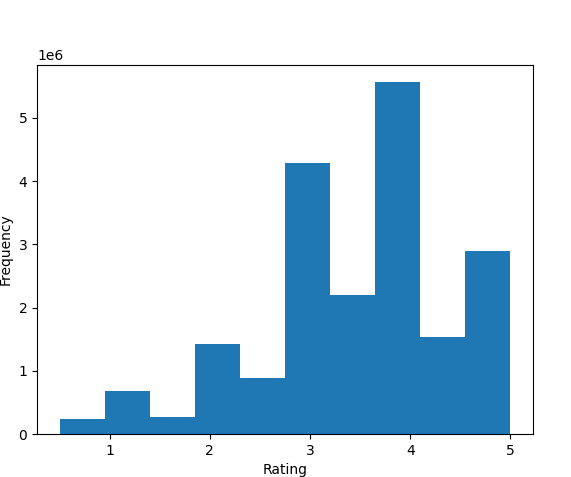
\includegraphics[width=0.8\textwidth]{pictures/movielens-20m-ratings-frequency}
\caption{Ratings frequency for MovieLens 20M}
\label{fg:movielens-20m-ratings-frequency}
\end{figure}
\begin{figure}[hbt!]
\centering
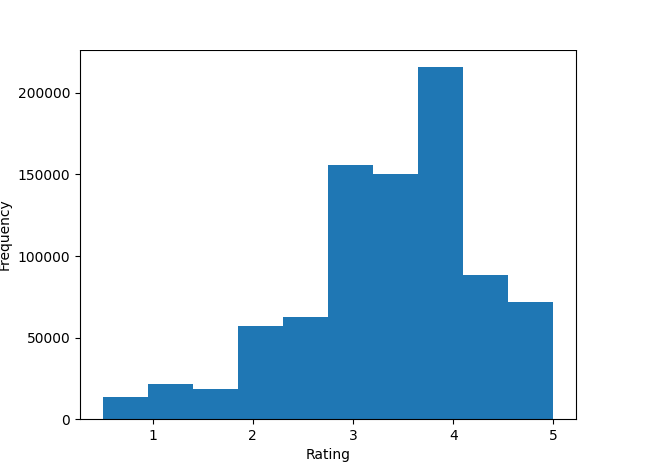
\includegraphics[width=0.9\textwidth]{pictures/movielens-hetrec-2011-ratings-frequency}
\caption{Ratings frequency for MovieLens Hetrec 2011}
\label{fg:movielens-hetrec-2011-ratings-frequency}
\end{figure}
\begin{figure}[hbt!]
\centering
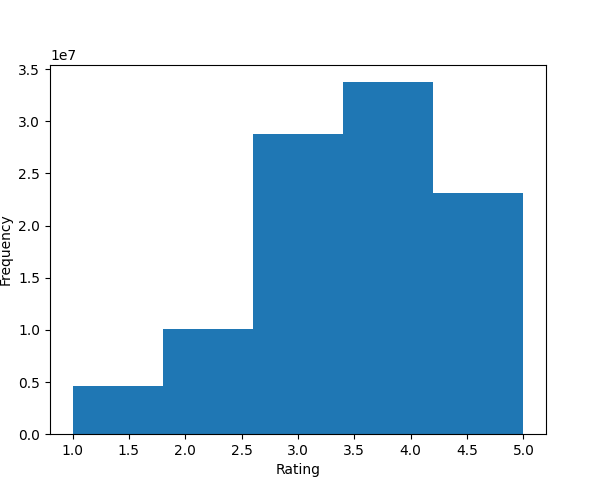
\includegraphics[width=0.8\textwidth]{pictures/netflix-prize-ratings-frequency}
\caption{Ratings frequency for Netflix Prize}
\label{fg:netflix-prize-ratings-frequency}
\end{figure}
\begin{figure}[hbt!]
\centering
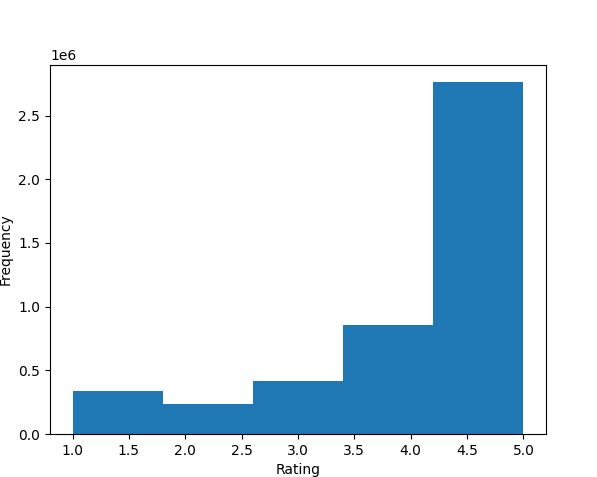
\includegraphics[width=0.8\textwidth]{pictures/amazon-movies-tv-series-ratings-frequency}
\caption{Ratings frequency for Amazon Movies TV Series}
\label{fg:amazon-movies-tv-series-ratings-frequency}
\end{figure}
\begin{table}[hbt]
\centering
\begin{tabulary}{1.0\textwidth}{|L|CCCC|}
\hline
\multicolumn{5}{|c|}{Source Domains} \\
\hline
& Density (\%) & Users & Items & Ratings \\
\hline
MovieLens 20M & 81.44 & 500 & 500 & 203610 \\
Netflix Prize & 56.77 & 500 & 500 & 141934 \\
\hline
\hline
\multicolumn{5}{|c|}{Target Domains} \\
\hline
& Density (\%) & Users & Items & Ratings \\
\hline
MovieLens Hetrec 2011 D. & 11.66 & 500 & 1000 & 58298 \\
MovieLens Hetrec 2011 S. & 2.93 & 500 & 1000 & 14627 \\
Netflix Prize D. & 11.53 & 500 & 1000 & 57656 \\
Netflix Prize S. & 3.78 & 500 & 1000 & 18904 \\
Amazon Movies TV Series D. & 10.21 & 500 & 1000 & 51048 \\
Amazon Movies TV Series S. & 2.88 & 500 & 1000 & 14416 \\
\hline
\end{tabulary}
\caption{Properties of the preprocessed datasets used in the experiments. `D.' and `S.' stand for dense and sparse.}
\end{table}
\label{tb:second-set-datasets-properties}
MovieLens 20M and Netflix Prize are preprocessed to extract very dense datasets to be used as source domain.\\
MovieLens Hetrec 2011, Netflix Prize and Amazon Movies TV Series are preprocessed to extract sparse and dense versions, both to be used as target domain.\\
Preprocessing for both source and target domains is performed in multiple iterations. First by removing users with a low amount of interactions, then by removing items with a low amount of interactions. Each missing rating of the source domain is filled with the average of ratings of its user.\\
Finally, the preprocessed datasets used in the experiments have the properties listed in \autoref{tb:second-set-datasets-properties}.\\
Each target dataset is split in train, validation and test sets. To do so, a random rating for each user is removed from the dataset and added to the validation set. The same is done for the test set, while the remaining ratings form the train set.


\subsection{Hyperparameters}

The set and optimized hyperparameters are the same described in \autoref{ss:first-set-datasets-hyperparameters}, except for the following:\\\\
$\texttt{transfer\_attempts} = 30$: the amount of attempts to find a local minimum for codebook transfer, as described in \autoref{ss:applied-codebook-transfer}.

\clearpage


\subsection{Results}

\begin{figure}[hbt!]
\centering
\begin{subfigure}{\textwidth}
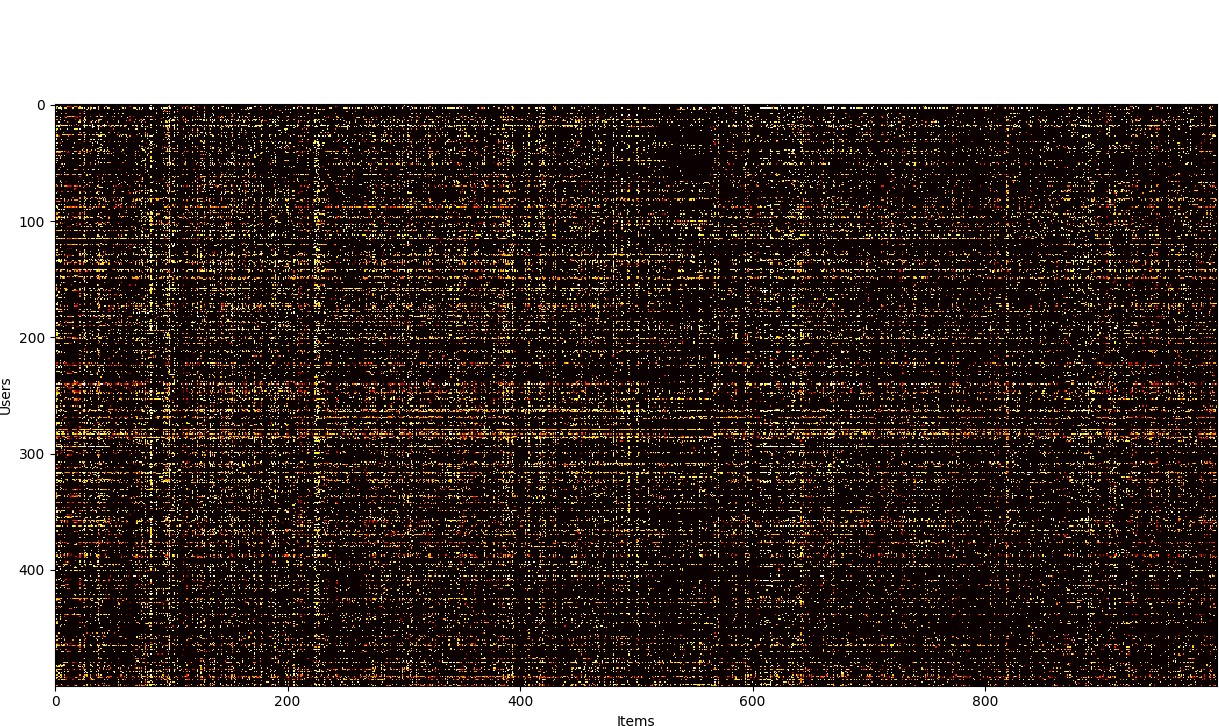
\includegraphics[width=\textwidth]{pictures/movielens-target}
\end{subfigure}
\begin{subfigure}{\textwidth}
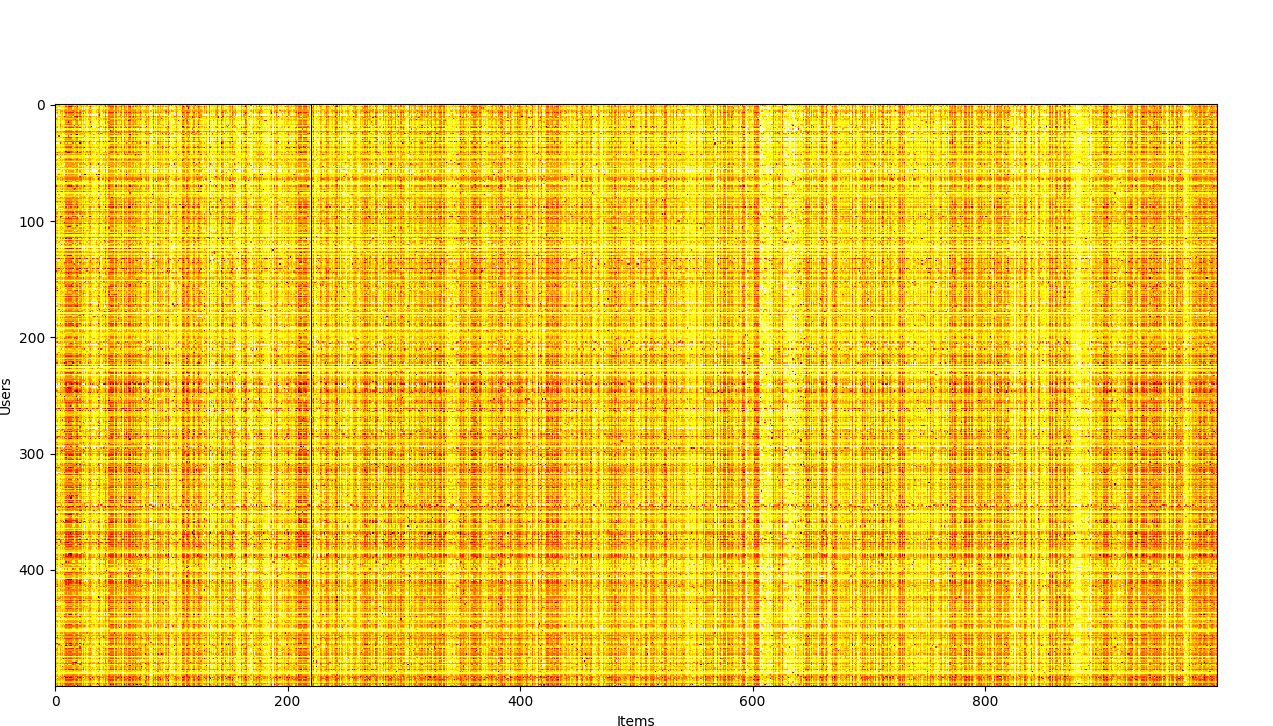
\includegraphics[width=\textwidth]{pictures/movielens-target-filled}
\end{subfigure}
\caption{Heatmap of the preprocessed MovieLens Hetrec 2011 Dense train set before and after the codebook transfer process performed with Netflix Prize as source domain. Low to high values are mapped to red to yellow color scale. Black dots represent missing ratings. The missing ratings in the filled target matrix represent users or items that could not be mapped to clusters during codebook construction.}
\end{figure}

\begin{table}[hbt]
\centering
\begin{tabulary}{\textwidth}{|L|CCC|}
\hline
\multicolumn{4}{|c|}{MovieLens 20M $\rightarrow$ Amazon Movies TV Series (Dense)} \\
\hline
\hline
Cut-off @20 & mAP & nDCG & Precision \\
\hline
TopPop & 0.0130 $\pm$ 0.0024 & 0.0219 $\pm$ 0.0043 & 0.0028 $\pm$ 0.0006 \\
Random & 0.0047 $\pm$ 0.0004 & 0.0098 $\pm$ 0.0009 & 0.0014 $\pm$ 0.0002 \\
kNN P. & 0.0242 $\pm$ 0.0036 & 0.0388 $\pm$ 0.0045 & 0.0046 $\pm$ 0.0004 \\
kNN C. & 0.0476 $\pm$ 0.0060 & 0.0713 $\pm$ 0.0063 & 0.0080 $\pm$ 0.0005 \\
targetCBT P. & 0.0094 $\pm$ 0.0015 & 0.0164 $\pm$ 0.0012 & 0.0021 $\pm$ 0.0002 \\
targetCBT C. & 0.0078 $\pm$ 0.0011 & 0.0147 $\pm$ 0.0011 & 0.0020 $\pm$ 0.0000 \\
\hline
CBT P. & 0.0073 $\pm$ 0.0027 & 0.0143 $\pm$ 0.0041 & 0.0020 $\pm$ 0.0005 \\
CBT C. & 0.0077 $\pm$ 0.0017 & 0.0151 $\pm$ 0.0028 & 0.0021 $\pm$ 0.0003 \\
\hline
\hline
Cut-off @20 & Recall & Gini Diversity & Item Coverage \\
\hline
TopPop & 0.0553 $\pm$ 0.0123 & 0.0289 $\pm$ 0.0000 & 0.0700 $\pm$ 0.0000 \\
Random & 0.0287 $\pm$ 0.0041 & 0.8175 $\pm$ 0.0001 &1.0000 $\pm$ 0.0000 \\
kNN P. & 0.0913 $\pm$ 0.0077 & 0.1151 $\pm$ 0.0602 & 0.4547 $\pm$ 0.1610 \\
kNN C. & 0.1593 $\pm$ 0.0093 & 0.4525 $\pm$ 0.1251 & 0.8973 $\pm$ 0.0942 \\
targetCBT P. & 0.0420 $\pm$ 0.0043 & 0.1713 $\pm$ 0.1252 & 0.5303 $\pm$ 0.2942 \\
targetCBT C. & 0.0407 $\pm$ 0.0009 & 0.0645 $\pm$ 0.0276 & 0.2917 $\pm$ 0.1655 \\
\hline
CBT P. & 0.0400 $\pm$ 0.0091 & 0.1035 $\pm$ 0.0648 & 0.4347 $\pm$ 0.2614 \\
CBT C. & 0.0427 $\pm$ 0.0066 & 0.0875 $\pm$ 0.0877 & 0.3103 $\pm$ 0.3583 \\
\hline
\end{tabulary}
\caption{Results of CBT experiment on preprocessed target dataset for cut-off @20 on Amazon Movies TV Series (Dense), with MovieLens 20M as source domain. `P.' and `C.' stand for Pearson and cosine similarity. Higher values are better.}
\end{table}

\begin{table}[hbt]
\centering
\begin{tabulary}{\textwidth}{|L|CCC|}
\hline
\multicolumn{4}{|c|}{MovieLens 20M $\rightarrow$ Amazon Movies TV Series (Sparse)} \\
\hline
\hline
Cut-off @20 & mAP & nDCG & Precision \\
\hline
TopPop & 0.0795 $\pm$ 0.0099 & 0.0988 $\pm$ 0.0095 & 0.0085 $\pm$ 0.0006 \\
Random & 0.0033 $\pm$ 0.0007 & 0.0066 $\pm$ 0.0008 & 0.0010 $\pm$ 0.0001 \\
kNN P. & 0.0748 $\pm$ 0.0146 & 0.0913 $\pm$ 0.0140 & 0.0075 $\pm$ 0.0006 \\
kNN C. & 0.0911 $\pm$ 0.0115 & 0.1120 $\pm$ 0.0119 & 0.0093 $\pm$ 0.0008 \\
targetCBT P. & 0.0132 $\pm$ 0.0062 & 0.0207 $\pm$ 0.0089 & 0.0024 $\pm$ 0.0010 \\
targetCBT C. & 0.0116 $\pm$ 0.0026 & 0.0188 $\pm$ 0.0025 & 0.0022 $\pm$ 0.0001 \\
\hline
CBT P. & 0.0624 $\pm$ 0.0060 & 0.0754 $\pm$ 0.0059 & 0.0062 $\pm$ 0.0003 \\
CBT C. & 0.0641 $\pm$ 0.0088 & 0.0757 $\pm$ 0.0100 & 0.0059 $\pm$ 0.0009 \\
\hline
\hline
Cut-off @20 & Recall & Gini Diversity & Item Coverage \\
\hline
TopPop & 0.1707 $\pm$ 0.0124 & 0.0241 $\pm$ 0.0000 & 0.0577 $\pm$ 0.0005 \\
Random & 0.0193 $\pm$ 0.0019 & 0.8188 $\pm$ 0.0002 &1.0000 $\pm$ 0.0000 \\
kNN P. & 0.1500 $\pm$ 0.0118 & 0.1131 $\pm$ 0.0120 & 0.5647 $\pm$ 0.0673 \\
kNN C. & 0.1867 $\pm$ 0.0165 & 0.0412 $\pm$ 0.0053 & 0.2293 $\pm$ 0.0394 \\
targetCBT P. & 0.0487 $\pm$ 0.0195 & 0.0858 $\pm$ 0.0295 & 0.3587 $\pm$ 0.0375 \\
targetCBT C. & 0.0447 $\pm$ 0.0025 & 0.0389 $\pm$ 0.0228 & 0.1390 $\pm$ 0.1280 \\
\hline
CBT P. & 0.1233 $\pm$ 0.0066 & 0.0261 $\pm$ 0.0012 & 0.0800 $\pm$ 0.0071 \\
CBT C. & 0.1180 $\pm$ 0.0170 & 0.0235 $\pm$ 0.0000 & 0.0590 $\pm$ 0.0008 \\
\hline
\end{tabulary}
\caption{Results of CBT experiment on preprocessed target dataset for cut-off @20 on Amazon Movies TV Series (Sparse), with MovieLens 20M as source domain. `P.' and `C.' stand for Pearson and cosine similarity. Higher values are better.}
\end{table}

\begin{table}[hbt]
\centering
\begin{tabulary}{\textwidth}{|L|CCC|}
\hline
\multicolumn{4}{|c|}{MovieLens 20M $\rightarrow$ Netflix Prize (Dense)} \\
\hline
\hline
Cut-off @20 & mAP & nDCG & Precision \\
\hline
TopPop & 0.1079 $\pm$ 0.0032 & 0.1565 $\pm$ 0.0028 & 0.0169 $\pm$ 0.0002 \\
Random & 0.0063 $\pm$ 0.0014 & 0.0115 $\pm$ 0.0029 & 0.0019 $\pm$ 0.0005 \\
kNN P. & 0.1181 $\pm$ 0.0070 & 0.1720 $\pm$ 0.0052 & 0.0186 $\pm$ 0.0002 \\
kNN C. & 0.1573 $\pm$ 0.0101 & 0.2160 $\pm$ 0.0107 & 0.0215 $\pm$ 0.000 \\
targetCBT P. & 0.0599 $\pm$ 0.0045 & 0.0930 $\pm$ 0.0056 & 0.0109 $\pm$ 0.0005 \\
targetCBT C. & 0.0588 $\pm$ 0.0048 & 0.0940 $\pm$ 0.0058 & 0.0113 $\pm$ 0.0005 \\
\hline
CBT P. & 0.0607 $\pm$ 0.0016 & 0.0941 $\pm$ 0.0045 & 0.0110 $\pm$ 0.0009 \\
CBT C. & 0.0546 $\pm$ 0.0040 & 0.0868 $\pm$ 0.0048 & 0.0104 $\pm$ 0.0005 \\
\hline
\hline
Cut-off @20 & Recall & Gini Diversity & Item Coverage \\
\hline
TopPop & 0.3307 $\pm$ 0.0034 & 0.0596 $\pm$ 0.0000 & 0.2263 $\pm$ 0.0012 \\
Random & 0.0307 $\pm$ 0.0096 & 0.8044 $\pm$ 0.0001 & 0.9990 $\pm$ 0.0000 \\
kNN P. & 0.3647 $\pm$ 0.0050 & 0.0731 $\pm$ 0.0041 & 0.3120 $\pm$ 0.0312 \\
kNN C. & 0.4227 $\pm$ 0.0105 & 0.1123 $\pm$ 0.0096 & 0.3883 $\pm$ 0.0357 \\
targetCBT P. & 0.2093 $\pm$ 0.0094 & 0.0845 $\pm$ 0.0425 & 0.3350 $\pm$ 0.1239 \\
targetCBT C. & 0.2180 $\pm$ 0.0102 & 0.0400 $\pm$ 0.0018 & 0.1733 $\pm$ 0.0493 \\
\hline
CBT P. & 0.2120 $\pm$ 0.0172 & 0.0749 $\pm$ 0.0342 & 0.3020 $\pm$ 0.1192 \\
CBT C. & 0.2000 $\pm$ 0.0091 & 0.0551 $\pm$ 0.0251 & 0.2797 $\pm$ 0.1982 \\
\hline
\end{tabulary}
\caption{Results of CBT experiment on preprocessed target dataset for cut-off @20 on Netflix Prize (Dense), with MovieLens 20M as source domain. `P.' and `C.' stand for Pearson and cosine similarity. Higher values are better.}
\end{table}

\begin{table}[hbt]
\centering
\begin{tabulary}{\textwidth}{|L|CCC|}
\hline
\multicolumn{4}{|c|}{MovieLens 20M $\rightarrow$ Netflix Prize (Sparse)} \\
\hline
\hline
Cut-off @20 & mAP & nDCG & Precision \\
\hline
TopPop & 0.1522 $\pm$ 0.0103 & 0.2197 $\pm$ 0.0115 & 0.0231 $\pm$ 0.0007 \\
Random & 0.0026 $\pm$ 0.0015 & 0.0045 $\pm$ 0.0012 & 0.0006 $\pm$ 0.0000 \\
kNN P. & 0.1604 $\pm$ 0.0112 & 0.2281 $\pm$ 0.0144 & 0.0235 $\pm$ 0.0012 \\
kNN C. & 0.1847 $\pm$ 0.0132 & 0.2552 $\pm$ 0.0172 & 0.0253 $\pm$ 0.0016 \\
targetCBT P. & 0.1260 $\pm$ 0.0132 & 0.1787 $\pm$ 0.0156 & 0.0182 $\pm$ 0.0013 \\
targetCBT C. & 0.1264 $\pm$ 0.0153 & 0.1792 $\pm$ 0.0185 & 0.0182 $\pm$ 0.0015 \\
\hline
CBT P. & 0.0870 $\pm$ 0.0053 & 0.1113 $\pm$ 0.0074 & 0.0097 $\pm$ 0.0011 \\
CBT C. & 0.1006 $\pm$ 0.0120 & 0.1325 $\pm$ 0.0140 & 0.0121 $\pm$ 0.0010 \\
\hline
\hline
Cut-off @20 & Recall & Gini Diversity & Item Coverage \\
\hline
TopPop & 0.4620 $\pm$ 0.0150 & 0.0389 $\pm$ 0.0000 & 0.1070 $\pm$ 0.0022 \\
Random & 0.0120 $\pm$ 0.0000 & 0.8141 $\pm$ 0.0001 &1.0000 $\pm$ 0.0000 \\
kNN P. & 0.4693 $\pm$ 0.0249 & 0.0457 $\pm$ 0.0023 & 0.1457 $\pm$ 0.0068 \\
kNN C. & 0.5060 $\pm$ 0.0326 & 0.0493 $\pm$ 0.0055 & 0.1453 $\pm$ 0.0330 \\
targetCBT P. & 0.3633 $\pm$ 0.0253 & 0.0369 $\pm$ 0.0004 & 0.1440 $\pm$ 0.0075 \\
targetCBT C. & 0.3640 $\pm$ 0.0300 & 0.0364 $\pm$ 0.0042 & 0.1350 $\pm$ 0.0806 \\
\hline
CBT P. & 0.1933 $\pm$ 0.0225 & 0.0258 $\pm$ 0.0020 & 0.0463 $\pm$ 0.0104 \\
CBT C. & 0.2413 $\pm$ 0.0207 & 0.0265 $\pm$ 0.0001 & 0.0440 $\pm$ 0.0024 \\
\hline
\end{tabulary}
\caption{Results of CBT experiment on preprocessed target dataset for cut-off @20 on Netflix Prize (Sparse), with MovieLens 20M as source domain. `P.' and `C.' stand for Pearson and cosine similarity. Higher values are better.}
\end{table}

\begin{table}[hbt]
\centering
\begin{tabulary}{\textwidth}{|L|CCC|}
\hline
\multicolumn{4}{|c|}{Netflix Prize $\rightarrow$ Amazon Movies TV Series (Dense)} \\
\hline
\hline
Cut-off @20 & mAP & nDCG & Precision \\
\hline
TopPop & 0.0142 $\pm$ 0.0044 & 0.0242 $\pm$ 0.0044 & 0.0031 $\pm$ 0.0003 \\
Random & 0.0046 $\pm$ 0.0018 & 0.0100 $\pm$ 0.0034 & 0.0015 $\pm$ 0.0004 \\
kNN P. & 0.0244 $\pm$ 0.0018 & 0.0403 $\pm$ 0.0025 & 0.0049 $\pm$ 0.0004 \\
kNN C. & 0.0422 $\pm$ 0.0096 & 0.0665 $\pm$ 0.0094 & 0.0077 $\pm$ 0.0004 \\
targetCBT P. & 0.0089 $\pm$ 0.0030 & 0.0155 $\pm$ 0.0041 & 0.0020 $\pm$ 0.0004 \\
targetCBT C. & 0.0096 $\pm$ 0.0004 & 0.0163 $\pm$ 0.0011 & 0.0021 $\pm$ 0.0002 \\
\hline
CBT P. & 0.0148 $\pm$ 0.0032 & 0.0261 $\pm$ 0.0044 & 0.0034 $\pm$ 0.0004 \\
CBT C. & 0.0099 $\pm$ 0.0008 & 0.0163 $\pm$ 0.0012 & 0.0020 $\pm$ 0.0002 \\
\hline
\hline
Cut-off @20 & Recall & Gini Diversity & Item Coverage \\
\hline
TopPop & 0.0613 $\pm$ 0.0066 & 0.0289 $\pm$ 0.0000 & 0.0707 $\pm$ 0.0005 \\
Random & 0.0300 $\pm$ 0.0086 & 0.8177 $\pm$ 0.0000 &1.0000 $\pm$ 0.0000 \\
kNN P. & 0.0987 $\pm$ 0.0074 & 0.0919 $\pm$ 0.0254 & 0.4273 $\pm$ 0.1022 \\
kNN C. & 0.1547 $\pm$ 0.0081 & 0.2891 $\pm$ 0.1283 & 0.7123 $\pm$ 0.1619 \\
targetCBT P. & 0.0400 $\pm$ 0.0086 & 0.2232 $\pm$ 0.1476 & 0.6063 $\pm$ 0.3553 \\
targetCBT C. & 0.0413 $\pm$ 0.0041 & 0.0470 $\pm$ 0.0300 & 0.2290 $\pm$ 0.2411 \\
\hline
CBT P. & 0.0680 $\pm$ 0.0086 & 0.1722 $\pm$ 0.1132 & 0.5517 $\pm$ 0.3176 \\
CBT C. & 0.0400 $\pm$ 0.0043 & 0.0525 $\pm$ 0.0372 & 0.2233 $\pm$ 0.2331 \\
\hline
\end{tabulary}
\caption{Results of CBT experiment on preprocessed target dataset for cut-off @20 on Amazon Movies TV Series (Dense), with Netflix Prize as source domain. `P.' and `C.' stand for Pearson and cosine similarity. Higher values are better.}
\end{table}

\begin{table}[hbt]
\centering
\begin{tabulary}{\textwidth}{|L|CCC|}
\hline
\multicolumn{4}{|c|}{Netflix Prize $\rightarrow$ Amazon Movies TV Series (Sparse)} \\
\hline
\hline
Cut-off @20 & mAP & nDCG & Precision \\
\hline
TopPop & 0.0922 $\pm$ 0.0131 & 0.1110 $\pm$ 0.0127 & 0.0090 $\pm$ 0.0006 \\
Random & 0.0047 $\pm$ 0.0015 & 0.0092 $\pm$ 0.0021 & 0.0013 $\pm$ 0.0002 \\
kNN P. & 0.0843 $\pm$ 0.0012 & 0.1039 $\pm$ 0.0043 & 0.0087 $\pm$ 0.0007 \\
kNN C. & 0.1014 $\pm$ 0.0090 & 0.1219 $\pm$ 0.0095 & 0.0097 $\pm$ 0.0008 \\
targetCBT P. & 0.0145 $\pm$ 0.0044 & 0.0244 $\pm$ 0.0047 & 0.0030 $\pm$ 0.0003 \\
targetCBT C. & 0.0143 $\pm$ 0.0038 & 0.0219 $\pm$ 0.0030 & 0.0025 $\pm$ 0.0000 \\
\hline
CBT P. & 0.0454 $\pm$ 0.0232 & 0.0625 $\pm$ 0.0206 & 0.0062 $\pm$ 0.0013 \\
CBT C. & 0.0574 $\pm$ 0.0232 & 0.0754 $\pm$ 0.0158 & 0.0071 $\pm$ 0.0006 \\
\hline
\hline
Cut-off @20 & Recall & Gini Diversity & Item Coverage \\
\hline
TopPop & 0.1807 $\pm$ 0.0123 & 0.0241 $\pm$ 0.0000 & 0.0577 $\pm$ 0.0005 \\
Random & 0.0253 $\pm$ 0.0050 & 0.8189 $\pm$ 0.0003 &1.0000 $\pm$ 0.0000 \\
kNN P. & 0.1740 $\pm$ 0.0142 & 0.1163 $\pm$ 0.0155 & 0.5670 $\pm$ 0.0634 \\
kNN C. & 0.1947 $\pm$ 0.0152 & 0.0443 $\pm$ 0.0120 & 0.2343 $\pm$ 0.0903 \\
targetCBT P. & 0.0607 $\pm$ 0.0062 & 0.0899 $\pm$ 0.0183 & 0.3613 $\pm$ 0.1444 \\
targetCBT C. & 0.0493 $\pm$ 0.0009 & 0.0449 $\pm$ 0.0317 & 0.1487 $\pm$ 0.1410 \\
\hline
CBT P. & 0.1233 $\pm$ 0.0253 & 0.0534 $\pm$ 0.0406 & 0.2203 $\pm$ 0.2056 \\
CBT C. & 0.1413 $\pm$ 0.0120 & 0.0235 $\pm$ 0.0000 & 0.0603 $\pm$ 0.0017 \\
\hline
\end{tabulary}
\caption{Results of CBT experiment on preprocessed target dataset for cut-off @20 on Amazon Movies TV Series (Sparse), with Netflix Prize as source domain. `P.' and `C.' stand for Pearson and cosine similarity. Higher values are better.}
\end{table}

\begin{table}[hbt]
\centering
\begin{tabulary}{\textwidth}{|L|CCC|}
\hline
\multicolumn{4}{|c|}{Netflix Prize $\rightarrow$ MovieLens Hetrec 2011 (Dense)} \\
\hline
\hline
Cut-off @20 & mAP & nDCG & Precision \\
\hline
TopPop & 0.0321 $\pm$ 0.0029 & 0.0528 $\pm$ 0.0042 & 0.0065 $\pm$ 0.0005 \\
Random & 0.0048 $\pm$ 0.0011 & 0.0093 $\pm$ 0.0023 & 0.0013 $\pm$ 0.0004 \\
kNN P. & 0.0377 $\pm$ 0.0032 & 0.0610 $\pm$ 0.0056 & 0.0074 $\pm$ 0.0007 \\
kNN C. & 0.0576 $\pm$ 0.0062 & 0.0914 $\pm$ 0.0043 & 0.0107 $\pm$ 0.0002 \\
targetCBT P. & 0.0230 $\pm$ 0.0058 & 0.0373 $\pm$ 0.0076 & 0.0045 $\pm$ 0.0008 \\
targetCBT C. & 0.0247 $\pm$ 0.0011 & 0.0387 $\pm$ 0.0031 & 0.0045 $\pm$ 0.0005 \\
\hline
CBT P. & 0.0247 $\pm$ 0.0014 & 0.0393 $\pm$ 0.0024 & 0.0047 $\pm$ 0.0006 \\
CBT C. & 0.0242 $\pm$ 0.0015 & 0.0382 $\pm$ 0.0042 & 0.0045 $\pm$ 0.0007 \\
\hline
\hline
Cut-off @20 & Recall & Gini Diversity & Item Coverage \\
\hline
TopPop & 0.1293 $\pm$ 0.0096 & 0.0398 $\pm$ 0.0000 & 0.1383 $\pm$ 0.0012 \\
Random & 0.0260 $\pm$ 0.0071 & 0.8118 $\pm$ 0.0002 &1.0000 $\pm$ 0.0000 \\
kNN P. & 0.1480 $\pm$ 0.0150 & 0.0609 $\pm$ 0.0121 & 0.2443 $\pm$ 0.0569 \\
kNN C. & 0.2147 $\pm$ 0.0041 & 0.1400 $\pm$ 0.0260 & 0.4757 $\pm$ 0.0748 \\
targetCBT P. & 0.0907 $\pm$ 0.0152 & 0.0671 $\pm$ 0.0487 & 0.2443 $\pm$ 0.1920 \\
targetCBT C. & 0.0907 $\pm$ 0.0106 & 0.0296 $\pm$ 0.0001 & 0.0813 $\pm$ 0.0005 \\
\hline
CBT P. & 0.0933 $\pm$ 0.0124 & 0.0413 $\pm$ 0.0163 & 0.1810 $\pm$ 0.1421 \\
CBT C. & 0.0900 $\pm$ 0.0140 & 0.0295 $\pm$ 0.0001 & 0.0797 $\pm$ 0.0009 \\
\hline
\end{tabulary}
\caption{Results of CBT experiment on preprocessed target dataset for cut-off @20 on MovieLens Hetrec 2011 (Dense), with Netflix Prize as source domain. `P.' and `C.' stand for Pearson and cosine similarity. Higher values are better.}
\end{table}

\begin{table}[hbt]
\centering
\begin{tabulary}{\textwidth}{|L|CCC|}
\hline
\multicolumn{4}{|c|}{Netflix Prize $\rightarrow$ MovieLens Hetrec 2011 (Sparse)} \\
\hline
\hline
Cut-off @20 & mAP & nDCG & Precision \\
\hline
TopPop & 0.0192 $\pm$ 0.0018 & 0.0313 $\pm$ 0.0025 & 0.0038 $\pm$ 0.0002 \\
Random & 0.0039 $\pm$ 0.0010 & 0.0083 $\pm$ 0.0013 & 0.0012 $\pm$ 0.0002 \\
kNN P. & 0.0232 $\pm$ 0.0032 & 0.0389 $\pm$ 0.0046 & 0.0048 $\pm$ 0.0005 \\
kNN C. & 0.0470 $\pm$ 0.0016 & 0.0735 $\pm$ 0.0030 & 0.0085 $\pm$ 0.0004 \\
targetCBT P. & 0.0161 $\pm$ 0.0006 & 0.0259 $\pm$ 0.0004 & 0.0031 $\pm$ 0.0002 \\
targetCBT C. & 0.0136 $\pm$ 0.0007 & 0.0233 $\pm$ 0.0021 & 0.0030 $\pm$ 0.0006 \\
\hline
CBT P. & 0.0069 $\pm$ 0.0031 & 0.0129 $\pm$ 0.0051 & 0.0017 $\pm$ 0.0007 \\
CBT C. & 0.0124 $\pm$ 0.0023 & 0.0206 $\pm$ 0.0020 & 0.0025 $\pm$ 0.0004 \\
\hline
\hline
Cut-off @20 & Recall & Gini Diversity & Item Coverage \\
\hline
TopPop & 0.0753 $\pm$ 0.0050 & 0.0234 $\pm$ 0.0000 & 0.0443 $\pm$ 0.0005 \\
Random & 0.0247 $\pm$ 0.0047 & 0.8236 $\pm$ 0.0002 &1.0000 $\pm$ 0.0000 \\
kNN P. & 0.0960 $\pm$ 0.0102 & 0.2712 $\pm$ 0.0113 & 0.8263 $\pm$ 0.0123 \\
kNN C. & 0.1700 $\pm$ 0.0082 & 0.2066 $\pm$ 0.0171 & 0.6763 $\pm$ 0.0189 \\
targetCBT P. & 0.0627 $\pm$ 0.0041 & 0.0773 $\pm$ 0.0164 & 0.4820 $\pm$ 0.0800 \\
targetCBT C. & 0.0593 $\pm$ 0.0123 & 0.0223 $\pm$ 0.0002 & 0.0343 $\pm$ 0.0005 \\
\hline
CBT P. & 0.0347 $\pm$ 0.0133 & 0.0459 $\pm$ 0.0164 & 0.1887 $\pm$ 0.0528 \\
CBT C. & 0.0507 $\pm$ 0.0081 & 0.0221 $\pm$ 0.0002 & 0.0350 $\pm$ 0.0014 \\
\hline
\end{tabulary}
\caption{Results of CBT experiment on preprocessed target dataset for cut-off @20 on MovieLens Hetrec 2011 (Sparse), with Netflix Prize as source domain. `P.' and `C.' stand for Pearson and cosine similarity. Higher values are better.}
\end{table}

\clearpage


\section{Experiments Summary}

While in a few dataset combinations CBT and kNN performances are not significantly different, in most of them CBT is outperformed in both ranking and accuracy metrics by simple kNN. Moreover, while on the first set of datasets CBT has better metrics than TopPop, in the second set of datasets it is generally outperformed by it. In addition to that, we consider the fact that CBT, when provided with a significant source matrix, is not consistently better than its baseline, which instead is provided with a fake source matrix, and it results in a better performance only in the first set of datasets. These results suggest that, at least between less dense source and target datasets, CBT is not capable of transferring knowledge.\par
It is also important to notice that CBT performs better in mAP the smaller the codebook, since most of the dataset combinations reach the optimal mAP when the user and item clusters are the minimum possible values. This result can lead us to three conclusions:
\begin{itemize}
\item The fact that Gini diversity is often inferior in CBT, compared to simple kNN, can be traced back to the low amount of ratings diversity in the filled target matrix, due to the small codebook.
\item The inverse proportion between mAP and codebook size is a sign that either the codebook creation or the codebook transfer phase fails in mapping clusters.
\item The performance of CBT heavily improves when filled ratings have low impact on the kNN phase and, as a consequence, its behavior is similar to the one of simple kNN without codebook transfer.
\end{itemize}